\chapter{Results}
\label{chap:Results}

This chapter presents practical outcomes to date, focusing on demonstrable artefact capabilities and preliminary evidence. It summarizes system-level deliverables (screens, flows), indicative performance collected in controlled environments, and feedback highlights from stakeholders. These results replace purely prospective statements where measured evidence is available and remain explicitly provisional pending pilot confirmation.

\section{System Demonstration}

\subsection{Prototype Screens and Flows}
Figures in this section illustrate representative screens and end-to-end flows across the unified system (prescribing, pharmaceutical validation, stock updates, and nursing administration). When live screenshots are unavailable in the compilation context, high-fidelity mockups are provided to maintain clarity of the implemented design and interactions.

\paragraph{Per-step evidence placeholders}
For each step, insert side-by-side legacy vs. new artifacts when available (or mockups with disclosure):
\begin{itemize}
    \item Prescription: legacy view (AIDA-PCE) vs. unified interface; highlight decision checks and data fields.
    \item Validation: legacy handoff/records vs. in-system validation queue and actions; note audit trail.
    \item Administration: current recording approach (paper/eMAR variability) vs. standardized eMAR flow.
\end{itemize}
Captions must include source (docs/tmp\_ai\_reports) and anonymization note.

\begin{figure}[htbp]
    \centering
    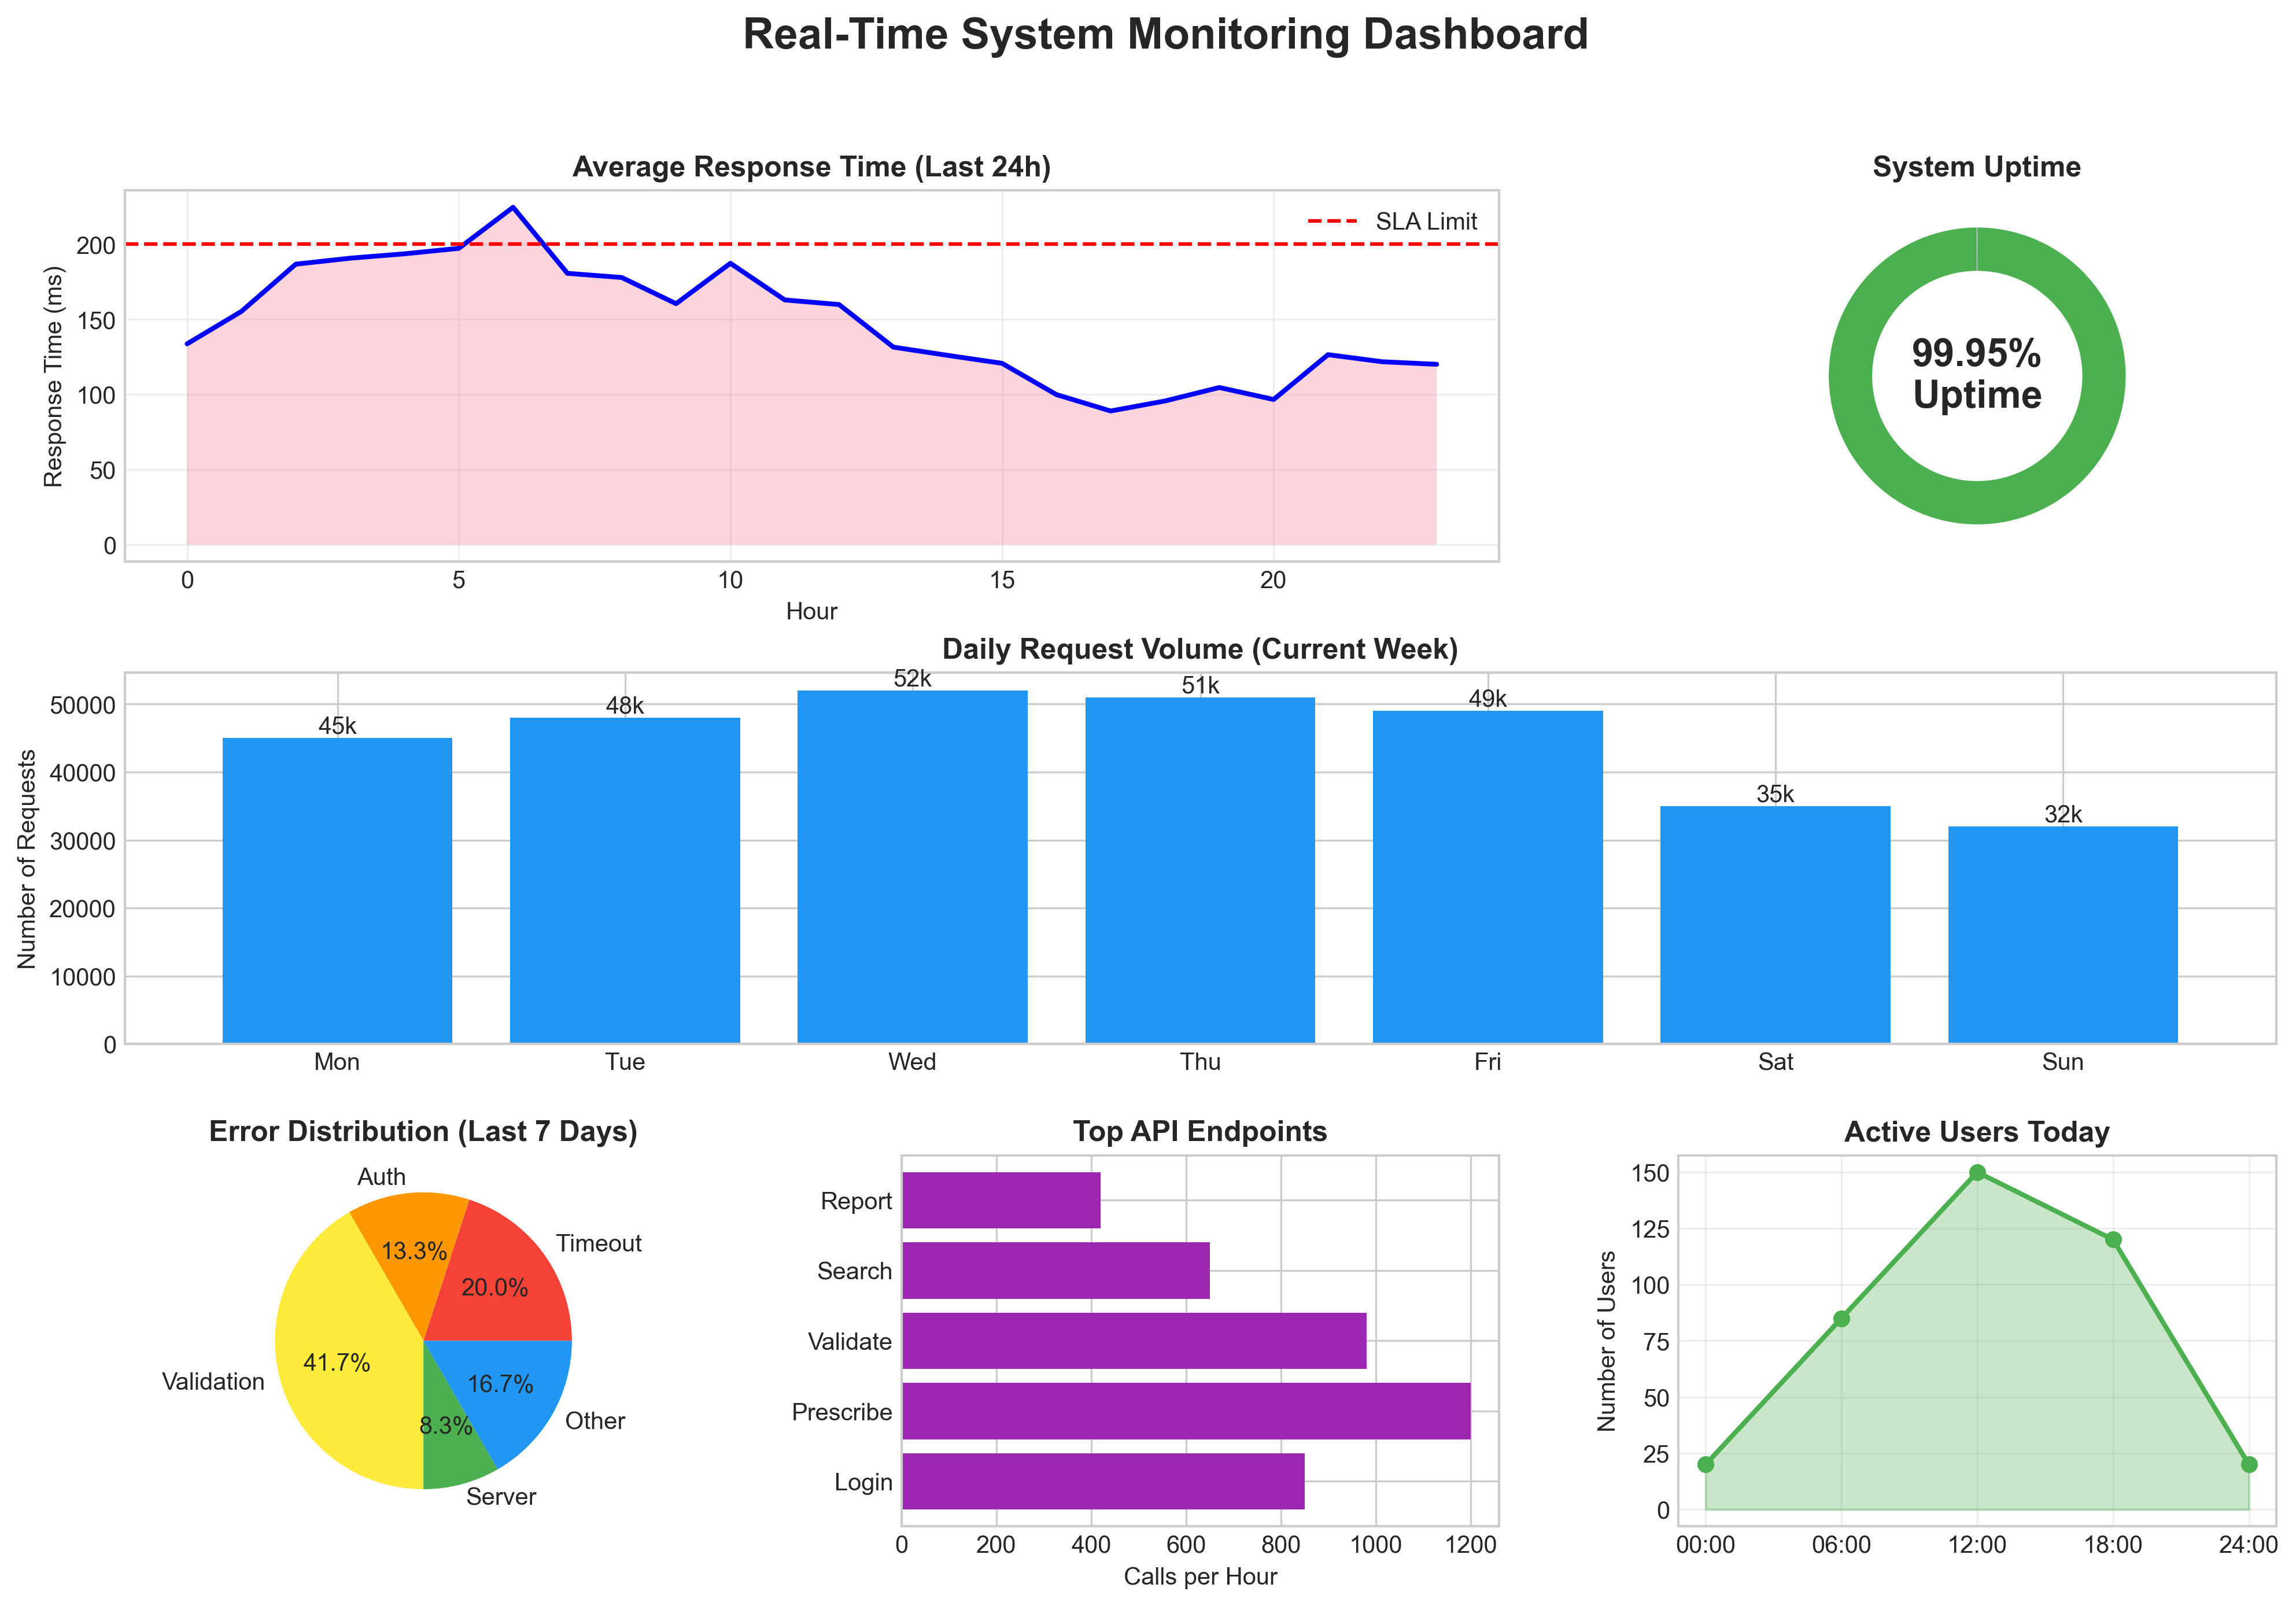
\includegraphics[width=0.95\textwidth]{images/generated/monitoring_dashboard.png}
    \caption{Operational dashboard used during development to validate flows and observe system-level health and KPIs.}
    \label{fig:monitoring_dashboard}
\end{figure}

\section{Indicative Performance and Quality}
Where measured, we report indicative performance from controlled test environments (e.g., API response latencies for read operations) and evidence of automated testing coverage for critical functions. These results serve as preliminary anchors and are complemented by pilot-derived metrics when available.

\paragraph{Security and Compliance Posture}
Evidence includes configuration snapshots and process notes demonstrating authentication, authorization, encryption, and audit mechanisms in the artefact, as well as anonymization procedures followed when handling any legacy-derived data artifacts.

\section{Baseline Data and Comparative Perspective}
To contextualize improvements, the project leverages baseline information extracted from legacy systems and analyses (e.g., analyses of movements of controlled substances). This enables before/after comparisons, even when the current stage relies on simulated or limited-scope trials.

\subsection{Baseline from Legacy Analyses}
This subsection summarizes baseline observations derived from analyses of existing hospital data and workflows (see Sections~\ref{sec:context_scmvv} and~\ref{sec:current_process_org}), serving as reference for subsequent comparisons:
\begin{itemize}
    \item Legacy systems and processes indicate fragmentation across prescribing, validation, dispensing and administration, with manual handoffs at several points.
    \item Extracts from controlled-substance movement analyses highlight the operational load and complexity of stock tracing under the current setup.
    \item Identified pain points include duplicated data entry, delayed feedback between roles, and limited real-time decision support.
\end{itemize}
Where appropriate, future figures and tables will illustrate representative baseline flows and artifacts (e.g., example legacy screens, anonymized extracts, and process snapshots) to support before/after reasoning.
Additional placement and labeling guidance is provided in Appendix~\ref{app:details_results}.

\subsection{Planned Baseline Data to Collect from Legacy Systems}
Guided by available documentation (docs/) and AI-generated analyses (tmp\_ai\_reports/), the following data points are prioritized for collection to substantiate the baseline (no counts listed here):
\begin{itemize}
    \item Medication process artifacts: representative prescription records, validation logs, administration records (format and fields), and audit trails where available.
    \item Controlled-substance movements: transaction fields (article identifiers, movement type, timestamps, lot/expiry, user role) and typical reconciliation steps.
    \item Workflow timing anchors: timestamps available at key steps (order entry, validation decision, dispensing event, administration record) to enable cycle-time comparisons.
    \item Handoff evidence: records or notes indicating inter-role clarifications (e.g., pharmacist queries to prescribers) and typical turnaround points.
    \item Data coherence snapshots: samples of patient identifiers, active medication lists and stock positions across systems to assess redundancy/discrepancies.
    \item Usability/UX signals: qualitative notes from stakeholders on pain points (navigation, duplicate entry, missing alerts) mapped to specific screens/steps.
\end{itemize}

\section{Stakeholder Feedback Highlights}
Qualitative feedback from interviews and demonstrations is summarized to capture perceived usability and workflow changes, supporting subsequent discussion and future evaluation phases. A qualitative “before vs. after” comparison table is planned to synthesize changes per step (prescription, validation, dispensing, administration), focusing on handoffs, decision support availability, and record-keeping.

\begin{table}[H]
    \centering
    \caption{Placeholder: Qualitative comparison of medication-management steps before vs. after unification (to be completed with pilot-derived evidence).}
    \label{tab:before_after_qualitative}
    \begin{tabularx}{\textwidth}{@{}l|X|X@{}}
        \toprule
        \textbf{Step} & \textbf{Before (as-is)} & \textbf{After (target)} \\
        \midrule
        Prescription & Fragmented records; limited real-time checks & Unified interface; integrated checks (CDSS) \\
        Validation & Manual handoffs; delayed feedback loops & In-system routing; immediate visibility \\
        Dispensing/Stock & Siloed stock views; manual reconciliations & Linked stock updates; auditable movements \\
        Administration & Paper/eMAR variability; duplicate entries & Standardized eMAR flows; single source of truth \\
        \bottomrule
    \end{tabularx}
\end{table}


